As mentioned in \fig{accessor}, a general flow of building recommender systems is (1) taking a list of user-item interactions, (2) applying certain mathematical operations, and (3) finding out the top-$k$ most promising list of items for a target user; \texttt{Recommendation.jl} provides standard interfaces \texttt{fit!()} and \texttt{recommend()} to undergo step (2) and (3), respectively. 

\begin{lstlisting}[language = Julia]
abstract type Recommender end

function fit!(recommender::Recommender; kwargs...)
end

function recommend(recommender::Recommender, 
                   user::Integer, topk::Integer, 
                   candidates::AbstractVector{T}
                  ) where {T<:Integer}
end
\end{lstlisting}

That is, among various pre-defined options we see in the following sections, we can choose an arbitrary recommender that inherits the abstract \texttt{Recommender} type. Meanwhile, by implementing a custom concrete subtype like \texttt{MyCustomModel} below and corresponding \texttt{fit!()} and \texttt{recommend()} functions, the developers can build a custom recommendation pipeline on the top of \texttt{Recommendation.jl}. The separation of common interfaces and actual algorithm implementation makes the package extensible.

\begin{lstlisting}[language = Julia]
struct MyCustomModel <: Recommender 
  data::DataAccessor
end
\end{lstlisting}

In the following sections, we review the basic recommendation algorithms \texttt{Recommendation.jl} natively supports. As previously explained, we delegate data manipulation to \texttt{DataAccessor}, and hence each of the recommendation models simply takes a \texttt{DataAccessor} instance, as well as some recommender-specific optional arguments, through its constructor to be initialized. The fact minimizes the gap between different recommender interfaces and maximizes the usability of \texttt{Recommendation.jl}.

\subsection{Non-Personalized Baselines}

First and foremost, recommender systems are not necessarily built by complex linear algebra or machine learning, and rule-based ``non-personalized'' recommenders are commonly used as a baseline method that derives reasonable recommendations. For instance, regardless of the target user's characteristics, a recommender \texttt{MostPopular(data::DataAccessor)} will return top-$k$ most popular items to every user, measured by the number of occurrences (i.e., popularity) in the whole user-item events:

\begin{lstlisting}[language = Julia]
recommender = MostPopular(data)

fit!(recommender)

# for user#4, recommend top-2 from all items
user, topk, candidates = 4, 2, collect(1:n_items)
recommend(recommender, user, topk, candidates)
# -> [item# => popularity] : [4 => 4.0, 6 => 4.0]
\end{lstlisting}

As of writing, the other non-personalized options implemented in the package will recommend items: that is most frequently co-occurred with a specific reference item (\texttt{CoOccurrence}), based on a percentage of observed \texttt{Event} values that are greater than a certain threshold (\texttt{ThresholdPercentage}), or based on a global mean of observed \texttt{Event} values (\texttt{UserMean}, \texttt{ItemMean}).

\subsection{Collaborative Filtering}
\label{sec:cf}

Collaborative filtering (CF) is one of the earliest recommendation techniques that was initially introduced in 1992 \cite{Goldberg1992}. The goal of the CF algorithm is to suggest new items for a particular user based on a similarity metric. From a user's perspective, CF assumes that users who behaved similarly on a service share common tastes for items. On the other hand, items which resemble each other are likely to be preferred by the same users.

\subsubsection{$k$-Nearest Neighbor}

A $k$-nearest neighbor ($k$-NN) approach, one of the simplest CF algorithms, runs two-fold. First, missing values in $R$ are predicted based on past observations. Here, a $(u, i)$ element between a target user $u$ and item $i$ is estimated by computing the similarities of users (items). Second, a recommender chooses top-$N$ items from the results of the prediction step.

Importantly, $k$-NN can be classified into a \textit{user-based} and \textit{item-based} algorithm. In a user-based algorithm, user-user similarities are computed for every pair of rows in $R$. By contrast, item-based CF stands on column-wise similarities between items. \fig{cf} illustrates how CF works on a user-item matrix $R$. The elements are ratings in a $[1, 5]$ range for each user-item pair, so $1$ and $2$ mean relatively negative feedback and vice versa. In the figure, users $a$ and $c$ seem to have similar tastes because both of them gave nearly identical feedback to the item $1$, $4$, and $6$. From an item-item perspective, items $4$ and $6$ are similarly rated by user $a$, $b$, and $c$.

\begin{figure}[htbp]
  \centering
  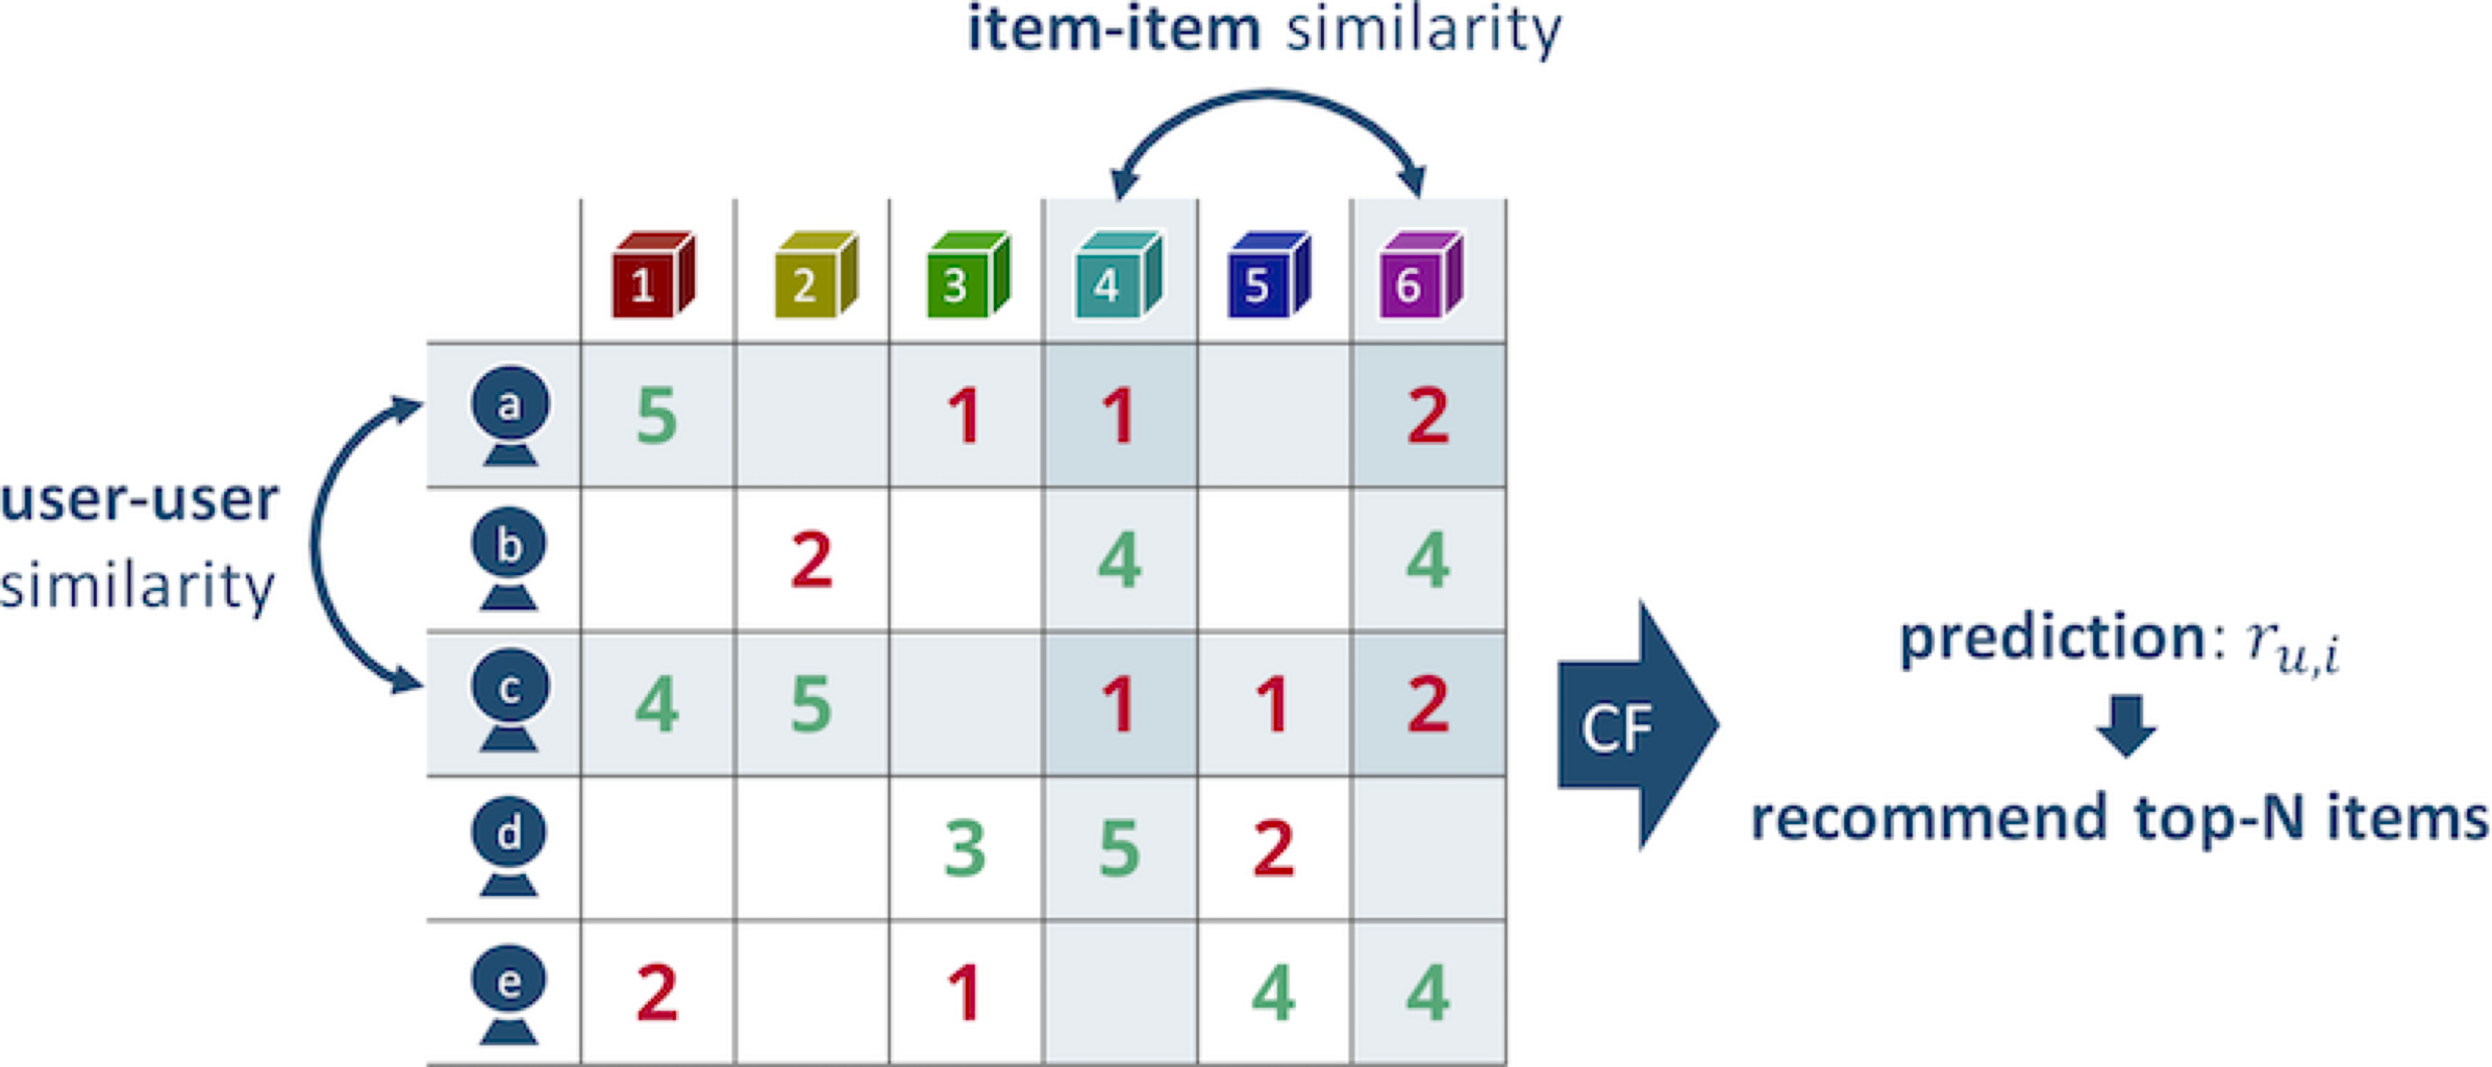
\includegraphics[width=1.0\linewidth]{images/cf.pdf}
  \caption{A schematic diagram of the $k$-NN-based recommender systems on a five-level rating matrix. This figure is based on Figure~1 in \cite{Sarwar2001} as a reference. For an active user $u$, his/her missing elements $r_{u,i}$ are estimated based on either user-user or item-item similarities, and a recommendation list contains the highest-scored items.}
  \label{fig:cf}
\end{figure}

To measure the similarities between rows (columns), the Pearson correlation and cosine similarity are widely used. For $d$-dimensional vectors $\mathbf{x}, \mathbf{y} \in \mathbb{R}^d$, the Pearson correlation $\mathrm{corr}(\mathbf{x}, \mathbf{y})$ and cosine similarity $\mathrm{cos}(\mathbf{x}, \mathbf{y})$ are respectively defined as:
$$
\mathrm{corr}(\mathbf{x}, \mathbf{y}) = \frac{\sum_i (x_{i} - \overline{x})(y_{i} - \overline{y})}{\sqrt{\sum_i (x_{i} - \overline{x})^2} \sqrt{\sum_i (y_{i} - \overline{y})^2}},
$$
$$
\mathrm{cos}(\mathbf{x}, \mathbf{y}) = \frac{\mathbf{x} \cdot \mathbf{y}}{\| \mathbf{x} \| \| \mathbf{y} \|} = \frac{\sum_i x_{i} y_{i}}{\sqrt{\sum_i x_{i}^2} \sqrt{\sum_i y_{i}^2}},
$$
where $\overline{x} = \frac{1}{d} \sum^d_{i=1} x_i$ and $\overline{y} = \frac{1}{d} \sum^d_{i=1} y_i$ denote mean values of the elements in a vector. Additionally, in the context of data mining, elements in $\mathbf{x}$ and $\mathbf{y}$ can be distributed on a different scale, so mean-centering of the vectors usually leads to better results \cite{Sarwar2001}. Note that cosine similarity between the mean-centered vectors, $\hat{\mathbf{x}} = (x_1 - \overline{x}, x_2 - \overline{x}, \dots, x_n - \overline{x})$ and $\hat{\mathbf{y}} = (y_1 - \overline{y}, y_2 - \overline{y}, \dots, y_n - \overline{y})$, is mathematically equivalent to the Pearson correlation $\mathrm{corr}(\mathbf{x}, \mathbf{y})$, meaning $\mathrm{cos}(\hat{\mathbf{x}}, \hat{\mathbf{y}}) = \mathrm{corr}(\mathbf{x}, \mathbf{y})$, and the following code snippet demonstrates its implementation in the Julia ecosystem.

\begin{lstlisting}[language = Julia]
import Statistics: mean
import LinearAlgebra: dot, norm

function similarity(x::AbstractVector,
                    y::AbstractVector)
    x_hat, y_hat = x .- mean(x), y .- mean(y)
    dot(x_hat, y_hat) / (
        norm(x_hat) * norm(y_hat))
end
\end{lstlisting}

Based on the similarity definition, user-based CF using the Pearson correlation \cite{Herlocker1999} sees $\mathbf{x}$ and $\mathbf{y}$ as two different rows in $R$, respectively, and gives weight to a user-user pair by the similarity. In the \texttt{fit!()} phase, the weights allow a recommender to (1) select the top-$k$ highest-weighted users (i.e., nearest neighbors) of a target user $u$, and (2) predict missing elements based on a mean value of neighbors' feedback. Ultimately, sorting items by the predicted values enables \texttt{recommend()} to generate a ranked list of recommended items for a user $u$. Simply put, a constructor of user-based CF in \texttt{Recommendation.jl} is as follows.

\begin{lstlisting}[language = Julia]
UserKNN(data::DataAccessor, n_neighbors::Integer)
\end{lstlisting}

It should be noted that user-based CF tends to be inefficient because gradually increasing massive users and their dynamic tastes require the model to frequently recompute the similarities. On the contrary, item properties are relatively stable compared to the users' tastes, and the number of items is generally smaller than the number of users. Hence, modeling item-item characteristics can be more promising in terms of both scalability and overall accuracy. In particular, the following recommender based on item-based CF \cite{Sarwar2001,Deshpande2004} provides an alternative way of predicting blanks in $R$ based on column-wise item-item similarities in the CF paradigm.

\begin{lstlisting}[language = Julia]
ItemKNN(data::DataAccessor, n_neighbors::Integer)
\end{lstlisting}

\subsubsection{Singular Value Decomposition}
\label{sec:svd}

Along with the development of the CF techniques, researchers noticed that handling the original huge user-item matrices is computationally expensive. Moreover, CF-based recommendation leads to overfitting to individual taste due to the sparsity of $R$. Thus, dimensionality reduction techniques were applied to the recommendation to capture more abstract preferences \cite{Sarwar2000}.

Singular value decomposition (SVD) is one of the most popular dimensionality reduction techniques that decomposes an $m$-by-$n$ matrix $A$ to $U \in \mathbb{R}^{m \times m}$, $\Sigma \in \mathbb{R}^{m \times n}$ and $V \in \mathbb{R}^{n \times n}$: 
\begin{align*}
\mathrm{SVD}(A) =& \ U \Sigma V^{\mathrm{T}} \\ 
= & \ \left[\mathbf{u}_1, \mathbf{u}_2, \cdots, \mathbf{u}_m\right] \cdot \mathrm{diag}\left(\sigma_1, \sigma_2, \dots, \sigma_{\min(m, n)}\right) \cdot \\
& \ \left[\mathbf{v}_1, \mathbf{v}_2, \cdots, \mathbf{v}_n\right]^{\mathrm{T}},
\end{align*}
by letting $\sigma_1 \geq \sigma_2 \geq \cdots \geq \sigma_{\min(m, n)} \geq 0$. An orthogonal matrix $U$ ($V$) is called left (right) singular vectors which represent characteristics of columns (rows) in $R$, and a diagonal matrix $\Sigma$ holds singular values on the diagonal elements as weights of each singular vector.

In practice, the most lower singular values of real-world matrices are very close to zero, and hence using only top-$k$ singular values $\Sigma_k \in \mathbb{R}^{k \times k}$ and corresponding singular vectors $U_k \in \mathbb{R}^{m \times k}$, $V_k \in \mathbb{R}^{n \times k}$ is sufficient to make a reasonable rank-$k$ approximation of a matrix $A$ as $\mathrm{SVD}_k(A) = U_k \Sigma_k V_k^{\mathrm{T}}$. It is mathematically proven that $\mathrm{SVD}_k(A)$ is the best rank-$k$ approximation of the matrix $A$ in both the spectral and Frobenius norm, where the spectral norm of a matrix equals its largest singular value.

\begin{figure}[htbp]
  \centering
  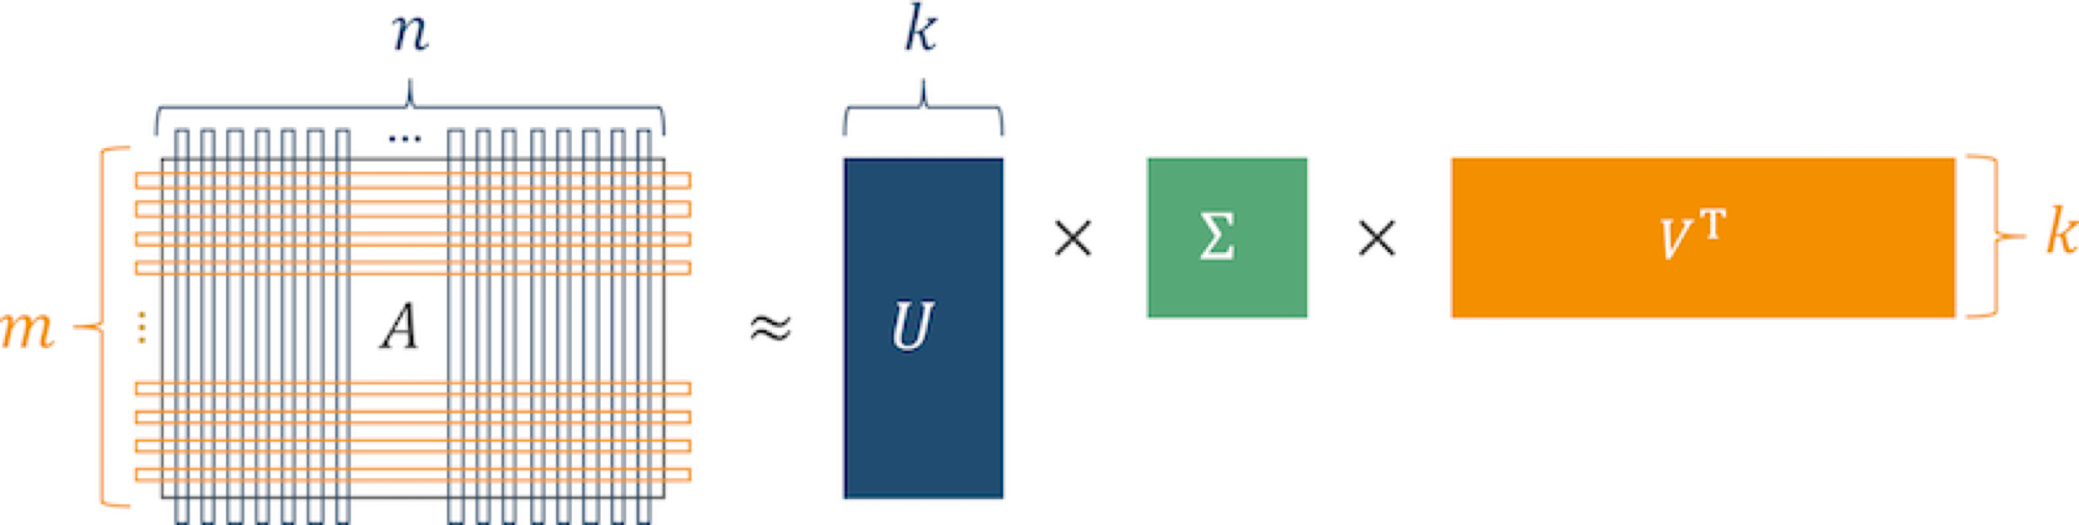
\includegraphics[width=1.0\linewidth]{images/svd.pdf}
  \caption{Rank-$k$ approximation based on SVD. $A \in \mathbb{R}^{m \times n}$ is decomposed into the rank-$k$ orthogonal matrices $U$ and $V$, and diagonal matrix $\Sigma$.}
  \label{fig:svd}
\end{figure}

Sarwar et~al. \cite{Sarwar2000} studied the use of SVD on user-item matrix $R \in \mathbb{R}^{|\mathcal{U}| \times |\mathcal{I}|}$. In a context of recommendation, $U_k \in \mathbb{R}^{|\mathcal{U}| \times k}$, $V \in \mathbb{R}^{|\mathcal{I}| \times k}$ and $\Sigma \in \mathbb{R}^{k \times k}$ are respectively seen as $k$ user/item feature vectors and corresponding weights. The idea of low-rank approximation that discards lower singular values intuitively works as \textit{compression} or \textit{denoising} of the original matrix; that is, each element in a rank-$k$ matrix $A_k$ holds the best \textit{compressed} (or \textit{denoised}) value of the original element in $A$. Thus, $R_k = \mathrm{SVD}_k(R)$, the best rank-$k$ approximation of $R$, holds underlying users' preferences the most. Once $R$ is decomposed into $U, \Sigma$ and $V$, a $(u, i)$ element of $R_k$ calculated by $\sum^k_{j=1} \sigma_j u_{u, j} v_{i, j}$ could be a prediction for the user-item pair. In the Julia ecosystem, the process can be implemented in a few lines of code with the standard \texttt{LinearAlgebra} library:

\begin{lstlisting}[language = Julia]
import LinearAlgebra: svd
F = svd(data.R)
U, S, Vt = F.U[:, 1:k], F.S[1:k], F.Vt[1:k, :]
# predict a value for an arbitrary user-item pair
r_k = dot(U[user, :] .* S, Vt[:, item])
\end{lstlisting}

\subsubsection{Matrix Factorization}

Even though dimensionality reduction is a promising approach to making an effective recommendation, the feasibility of SVD is still questionable due to the computational cost of decomposition and the need for uncertain preliminary work such as missing value imputation and searching an optimal $k$. As a result, a new technique generally called matrix factorization (MF) was introduced \cite{Koren2009} as an alternative.

The initial MF technique was invented by Funk \cite{Funk2006} during the Netflix Prize \cite{Bennett07thenetflix}, and the method is also known as \textit{regularized SVD} because it can be seen as an extension of the conventional SVD-based recommendation that gives an efficient approximation of the original SVD. The basic idea of MF is to factorize a user-item matrix $R$ to a user-factored matrix $P \in \mathbb{R}^{|\mathcal{U}| \times k}$ and item factored matrix $Q \in \mathbb{R}^{|\mathcal{I}| \times k}$, by solving the following minimization problem for a set of observed user-item interactions $\mathcal{S} = \{(u, i) \in \mathcal{U} \times \mathcal{I}\}$:
$$
  \min_{P, Q} \sum_{(u, i) \in \mathcal{S}} \left( r_{u,i} - \mathbf{p}_u^{\mathrm{T}} \mathbf{q}_i \right)^2 + \lambda \ (\|\mathbf{p}_u\|^2 + \|\mathbf{q}_i\|^2),
$$
where $\mathbf{p}_u, \mathbf{q}_i \in \mathbb{R}^k$ are respectively a factorized user and item vector, and $\lambda$ is a regularization parameter to avoid overfitting. Inside of \texttt{fit!()}, an optimal solution can be found by using optimization techniques such as stochastic gradient descent (SGD).

\begin{lstlisting}[language = Julia]
struct MatrixFactorization <: Recommender
    data::DataAccessor
    n_factors::Integer
    P::AbstractMatrix
    Q::AbstractMatrix
end
\end{lstlisting}

Eventually, $R$ is approximated by $PQ^{\mathrm{T}}$ as shown in \fig{mf}, and a recommender can rank items by the prediction. Notice that mathematically tractable properties of SVD such as orthogonality of factored matrices will be lost for approximation.

\begin{figure}[htbp]
  \centering
  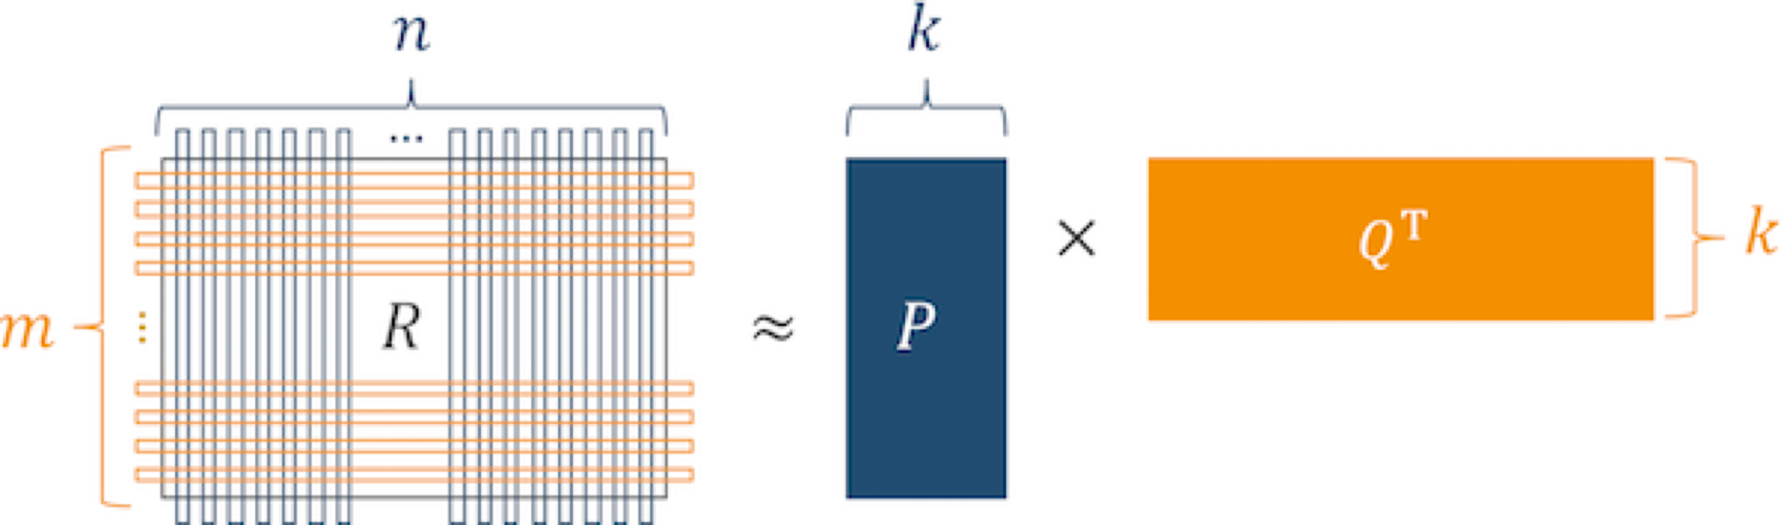
\includegraphics[width=0.8\linewidth]{images/mf.pdf}
  \caption{MF for an $m$-by-$n$ rating matrix $R$. Unlike SVD, singular values in $\Sigma$ are considered to be embedded in the factored matrices.}
  \label{fig:mf}
\end{figure}

MF is attractive in terms of not only efficiency but extensibility. Since prediction for each user-item pair can be written by a simple vector product as $r_{u,i} = \mathbf{p}_u^{\mathrm{T}} \mathbf{q}_i$, incorporating different features (e.g., biases and temporal factors) into the model as linear combinations is straightforward. For example, let $\mu$ be a global mean of all elements in $R$, and $b_u, b_i$ be respectively a user and item bias term. Here, we assume that each observation can be represented as $r_{u,i} = \mu + b_u + b_i + \mathbf{p}_u^{\mathrm{T}} \mathbf{q}_i$. This formulation is known as biased MF \cite{Koren2009}, and it is possible to capture more information than the original MF even on the same set of events $\mathcal{S}$. There are also other advanced methods such as tensor factorization \cite{Karatzoglou2010} that require higher dimensionality and a more costly optimization scheme to enrich MF.

Meanwhile, there are different options for loss functions to optimize MF. To give an example, Chen et~al. \cite{Chen2011} showed various types of features and loss functions which can be incorporated into an MF scheme. An appropriate choice of their combinations is likely to lead to surprisingly better accuracy compared to the classical MF, and \texttt{Recommendation.jl} currently supports Bayesian personalized ranking (BPR) loss \cite{10.5555/1795114.1795167} as an alternative option via \texttt{BPRMatrixFactorization <: Recommender}.

\subsection{Factorization Machines}

Beyond numerous discussions about MF, factorization machines (FMs) have been recently developed as their generalized model. In contrast to MF, FMs are formulated by an equation that is similar to polynomial regression, and the model can be applied to all regression, classification, and ranking problems depending on a choice of the loss function with or without SGD-based optimization.

First of all, for an input vector $\mathbf{x} \in \mathbb{R}^d$, let us imagine the following second-order polynomial model parameterized by $w_0 \in \mathbb{R}$, $\mathbf{w} \in \mathbb{R}^d$ as: $\hat{y}(\mathbf{x}) := w_0 + \mathbf{w}^{\mathrm{T}} \mathbf{x} + \sum_{i=1}^d \sum_{j=i}^d w_{i,j} x_i x_j,$ where $w_{i,j}$ is an element in a symmetric matrix $W \in \mathbb{R}^{d \times d}$, and it indicates a weight of $x_i x_j$, an interaction between the $i$-th and $j$-th element in $\mathbf{x}$. Here, FMs assume that $W$ can be approximated by a low-rank matrix $V \in \mathbb{R}^{d \times k}$ for $k < d$, and the weights are replaced with inner products of $k$ dimensional vectors as $w_{i, j} \approx \mathbf{v}_i^{\mathrm{T}} \mathbf{v}_j$ for $\mathbf{v}_1, \cdots, \mathbf{v}_d \in \mathbb{R}^k$. As a result, the formulation of the FM model is:
\begin{equation}
\hat{y}^{\mathrm{FM}}(\mathbf{x}) := \underbrace{w_0}_{\textbf{global bias}} + \underbrace{\mathbf{w}^{\mathrm{T}} \mathbf{x}_{ }}_{\textbf{linear}} + \sum_{i=1}^d \sum_{j=i}^d \underbrace{\mathbf{v}_i^{\mathrm{T}} \mathbf{v}_j}_{\textbf{interaction}} x_i x_j.
\label{eq:FMs}
\end{equation}
Several studies \cite{Geuens2015,Rendle2012-1,Rendle2012-3} prove that the flexibility of feature representations $\mathbf{x}$ is one of the most important characteristics that makes FMs versatile. The code snippet below demonstrates how a concatenated input vector is created with \texttt{Recommendation.jl}'s utility function \texttt{onehot()}.

\begin{lstlisting}[language = Julia]
x = vcat(
    onehot(1, collect(1:n_users)), # user ID
    onehot(3, collect(1:n_items)), # item ID
    2.5, # rating
    # ...
    onehot("Weekly", # email preference
          ["Daily", "Weekly", "Monthly", missing]),
    onehot(2, collect(1:7)) # day of week
)
\end{lstlisting}

Note that Rendle \cite{Rendle2012-1} specially referred to \eq{FMs} as \textit{second-order} FMs as a specific case that $p=2$ of the following $p$-th order FMs:
\begin{align*}
\hat{y}^{\mathrm{FM}^{(p)}}(\mathbf{x}) &:= w_0 + \mathbf{w}^{\mathrm{T}} \mathbf{x} \\ &+ \sum^p_{\ell=2} \sum^d_{j_1 = 1} \cdots \sum^d_{j_p = j_{p-1} + 1} \left( \prod^{\ell}_{i=1} x_{j_i} \right) \sum^{k_{\ell}}_{f=1} \prod^{\ell}_{i=1} v_{j_i,f},
\end{align*}
with the model parameters $w_0 \in \mathbb{R}, \ \mathbf{w} \in \mathbb{R}^d, \ V_{\ell} \in \mathbb{R}^{d \times k_{\ell}},$ where $\ell \in \{2, \cdots, p\}$. Although the higher-order FMs are attractive to capturing more complex underlying concepts from dynamic data, the computational cost should become more expensive accordingly. In favor of balancing the algorithmic sophistication and its efficiency, \texttt{Recommendation.jl} only considers the second-order model trained by SGD for the time being.

\begin{lstlisting}[language = Julia]
struct FactorizationMachines <: Recommender
    data::DataAccessor
    p::Integer
    n_factors::Integer
    w0::Base.RefValue{Float64} # mutable for fit!()
    w::AbstractVector
    V::AbstractMatrix
end
\end{lstlisting}

\subsection{Content-Based Filtering}

All techniques introduced so far rely on users' historical behavior on a service, but these kinds of recommenders easily face a challenge so-called \textit{cold-start} when it comes to recommending new items (for new users) that do not have a sufficient amount of historical data to capture meaningful information. To work around the difficulty, content-based recommender systems \cite{Lops2011} are likely to be preferred in reality.

Most importantly, content-based recommenders make a recommendation without using the other users' feedback. In particular, a content-based approach gives scores to items based on two kinds of information: item model and (static) user preference. To model the items, an item-attribute matrix is defined as $I \in \mathbb{R}^{|\mathcal{I}| \times |\mathcal{A}|}$, where $\mathcal{A}$ is a set of item attributes. Meanwhile, user attributes can be captured through \texttt{DataAccessor}'s \texttt{user\_attributes} property, which is independent of what kind of \texttt{Event}s a system has observed.

From a practical perspective, choosing a set of attributes $\mathcal{A}$ is an essential problem to launch a content-based recommender successfully. In fact, there tend to be numerous candidates on a real-world dataset such as item category and brand, but using too many attributes may increase the sparsity and complexity of the vectors, which ends up with poor recommendation performance. With that in mind, one of the most well-studied types of attribute \texttt{Recommendation.jl} also supports is ``term''. More concretely, each item is represented by a set of words, and the items are modeled by TF-IDF weighting \cite{Manning2008}. For instance, if we like to recommend web pages to users, we first need to parse sentences on a page and then construct a vector based on the frequency of each term as:

\begin{equation*}
  I=
  \begin{blockarray}{*{5}{c} l}
    \begin{block}{*{5}{>{$\footnotesize}c<{$}} l}
      apple & banana & candy & $\cdots$ & zoo & \\
    \end{block}
    \begin{block}{[*{5}{c}]>{$\footnotesize}l<{$}}
      3 & 2 & 0 & \cdots & 5 \bigstrut[t]& page\#1 \\
      1 & 0 & 0 & \cdots & 1 & page\#2 \\
      \vdots & \vdots & \vdots & \ddots & \vdots & \vdots \\
      2 & 1 & 8 & \cdots & 0 & page\#N \\
    \end{block}
  \end{blockarray}
\end{equation*}

In the case of our item-word matrices, for a given item $i$, term frequency (TF) for a term $t$ is defined as $\mathrm{tf}(t, i) = \frac{n_{t,i}}{N_i},$ where $n_{t,i}$ denotes an $(i, t)$ element in $I$, and $N_i$ is the total number of words that an item $i$ contains. Meanwhile, inverse document frequency (IDF) is computed over $M$ items as $\mathrm{idf}(t) = \log \frac{M}{\mathrm{df}(t)} + 1,$ where $\mathrm{df}(t)$ counts the number of items which associate with a term $t$. Finally, each item-term pair is weighted by: $\mathrm{tf}(t, i) \cdot \mathrm{idf}(t)$ in the TF-IDF scheme. 

Since there are several variations of how to calculate $\mathrm{tf}(t, i)$ and $\mathrm{idf}(t)$, \texttt{Recommendation.jl} requires users to pre-compute these numbers to maximize the feasibility of the recommender:

\begin{lstlisting}[language = Julia]
struct TFIDF <: Recommender
    data::DataAccessor
    tf::AbstractMatrix
    idf::AbstractMatrix
end
\end{lstlisting}

% If the features were chosen appropriately, content-based recommenders could work well even in challenging settings that cannot be handled by conventional recommenders. To give an example, when a new item is added to a system, making a reasonable prediction for the item is impossible by using classical approaches such as CF. By contrast, since content-based recommenders only require the attributes of items, new items can show up in a recommendation list with an equal chance to the old items. Furthermore, explaining the results of content-based recommendations is possible because the attributes are manually selected by humans.
